\documentclass[conference]{IEEEtran}
% Some Computer Society conferences also require the compsoc mode option,
% but others use the standard conference format.
%
% If IEEEtran.cls has not been installed into the LaTeX system files,
% manually specify the path to it like:
% \documentclass[conference]{../sty/IEEEtran}


% Some very useful LaTeX packages include:
% (uncomment the ones you want to load)


% *** MISC UTILITY PACKAGES ***
%
%\usepackage{ifpdf}
% Heiko Oberdiek's ifpdf.sty is very useful if you need conditional
% compilation based on whether the output is pdf or dvi.
% usage:
% \ifpdf
%   % pdf code
% \else
%   % dvi code
% \fi
% The latest version of ifpdf.sty can be obtained from:
% http://www.ctan.org/pkg/ifpdf
% Also, note that IEEEtran.cls V1.7 and later provides a builtin
% \ifCLASSINFOpdf conditional that works the same way.
% When switching from latex to pdflatex and vice-versa, the compiler may
% have to be run twice to clear warning/error messages.
\usepackage{enumitem}
\usepackage{siunitx}
\usepackage{multicol}
\usepackage{caption}
\usepackage{amsfonts}



% *** CITATION PACKAGES ***
%
\usepackage{cite}
% cite.sty was written by Donald Arseneau
% V1.6 and later of IEEEtran pre-defines the format of the cite.sty package
% \cite{} output to follow that of the IEEE. Loading the cite package will
% result in citation numbers being automatically sorted and properly
% "compressed/ranged". e.g., [1], [9], [2], [7], [5], [6] without using
% cite.sty will become [1], [2], [5]--[7], [9] using cite.sty. cite.sty's
% \cite will automatically add leading space, if needed. Use cite.sty's
% noadjust option (cite.sty V3.8 and later) if you want to turn this off
% such as if a citation ever needs to be enclosed in parenthesis.
% cite.sty is already installed on most LaTeX systems. Be sure and use
% version 5.0 (2009-03-20) and later if using hyperref.sty.
% The latest version can be obtained at:
% http://www.ctan.org/pkg/cite
% The documentation is contained in the cite.sty file itself.




% *** GRAPHICS RELATED PACKAGES ***
\usepackage{graphicx}
\graphicspath{{../../assets}}




% *** MATH PACKAGES ***
%
\usepackage{amsmath}
% A popular package from the American Mathematical Society that provides
% many useful and powerful commands for dealing with mathematics.
%
% Note that the amsmath package sets \interdisplaylinepenalty to 10000
% thus preventing page breaks from occurring within multiline equations. Use:
%\interdisplaylinepenalty=2500
% after loading amsmath to restore such page breaks as IEEEtran.cls normally
% does. amsmath.sty is already installed on most LaTeX systems. The latest
% version and documentation can be obtained at:
% http://www.ctan.org/pkg/amsmath




% *** SPECIALIZED LIST PACKAGES ***
%
\usepackage{algorithmic}
% algorithmic.sty was written by Peter Williams and Rogerio Brito.
% This package provides an algorithmic environment fo describing algorithms.
% You can use the algorithmic environment in-text or within a figure
% environment to provide for a floating algorithm. Do NOT use the algorithm
% floating environment provided by algorithm.sty (by the same authors) or
% algorithm2e.sty (by Christophe Fiorio) as the IEEE does not use dedicated
% algorithm float types and packages that provide these will not provide
% correct IEEE style captions. The latest version and documentation of
% algorithmic.sty can be obtained at:
% http://www.ctan.org/pkg/algorithms
% Also of interest may be the (relatively newer and more customizable)
% algorithmicx.sty package by Szasz Janos:
% http://www.ctan.org/pkg/algorithmicx




% *** ALIGNMENT PACKAGES ***
%
\usepackage{array}
% Frank Mittelbach's and David Carlisle's array.sty patches and improves
% the standard LaTeX2e array and tabular environments to provide better
% appearance and additional user controls. As the default LaTeX2e table
% generation code is lacking to the point of almost being broken with
% respect to the quality of the end results, all users are strongly
% advised to use an enhanced (at the very least that provided by array.sty)
% set of table tools. array.sty is already installed on most systems. The
% latest version and documentation can be obtained at:
% http://www.ctan.org/pkg/array


% IEEEtran contains the IEEEeqnarray family of commands that can be used to
% generate multiline equations as well as matrices, tables, etc., of high
% quality.




% *** SUBFIGURE PACKAGES ***
\ifCLASSOPTIONcompsoc
 \usepackage[caption=false,font=normalsize,labelfont=sf,textfont=sf]{subfig}
\else
 \usepackage[caption=false,font=footnotesize]{subfig}
\fi
% subfig.sty, written by Steven Douglas Cochran, is the modern replacement
% for subfigure.sty, the latter of which is no longer maintained and is
% incompatible with some LaTeX packages including fixltx2e. However,
% subfig.sty requires and automatically loads Axel Sommerfeldt's caption.sty
% which will override IEEEtran.cls' handling of captions and this will result
% in non-IEEE style figure/table captions. To prevent this problem, be sure
% and invoke subfig.sty's "caption=false" package option (available since
% subfig.sty version 1.3, 2005/06/28) as this is will preserve IEEEtran.cls
% handling of captions.
% Note that the Computer Society format requires a larger sans serif font
% than the serif footnote size font used in traditional IEEE formatting
% and thus the need to invoke different subfig.sty package options depending
% on whether compsoc mode has been enabled.
%
% The latest version and documentation of subfig.sty can be obtained at:
% http://www.ctan.org/pkg/subfig




% *** FLOAT PACKAGES ***
%
%\usepackage{fixltx2e}
% fixltx2e, the successor to the earlier fix2col.sty, was written by
% Frank Mittelbach and David Carlisle. This package corrects a few problems
% in the LaTeX2e kernel, the most notable of which is that in current
% LaTeX2e releases, the ordering of single and double column floats is not
% guaranteed to be preserved. Thus, an unpatched LaTeX2e can allow a
% single column figure to be placed prior to an earlier double column
% figure.
% Be aware that LaTeX2e kernels dated 2015 and later have fixltx2e.sty's
% corrections already built into the system in which case a warning will
% be issued if an attempt is made to load fixltx2e.sty as it is no longer
% needed.
% The latest version and documentation can be found at:
% http://www.ctan.org/pkg/fixltx2e


%\usepackage{stfloats}
% stfloats.sty was written by Sigitas Tolusis. This package gives LaTeX2e
% the ability to do double column floats at the bottom of the page as well
% as the top. (e.g., "\begin{figure*}[!b]" is not normally possible in
% LaTeX2e). It also provides a command:
%\fnbelowfloat
% to enable the placement of footnotes below bottom floats (the standard
% LaTeX2e kernel puts them above bottom floats). This is an invasive package
% which rewrites many portions of the LaTeX2e float routines. It may not work
% with other packages that modify the LaTeX2e float routines. The latest
% version and documentation can be obtained at:
% http://www.ctan.org/pkg/stfloats
% Do not use the stfloats baselinefloat ability as the IEEE does not allow
% \baselineskip to stretch. Authors submitting work to the IEEE should note
% that the IEEE rarely uses double column equations and that authors should try
% to avoid such use. Do not be tempted to use the cuted.sty or midfloat.sty
% packages (also by Sigitas Tolusis) as the IEEE does not format its papers in
% such ways.
% Do not attempt to use stfloats with fixltx2e as they are incompatible.
% Instead, use Morten Hogholm'a dblfloatfix which combines the features
% of both fixltx2e and stfloats:
%
% \usepackage{dblfloatfix}
\usepackage{float}
% The latest version can be found at:
% http://www.ctan.org/pkg/dblfloatfix




% *** PDF, URL AND HYPERLINK PACKAGES ***
%
\usepackage{url}
% url.sty was written by Donald Arseneau. It provides better support for
% handling and breaking URLs. url.sty is already installed on most LaTeX
% systems. The latest version and documentation can be obtained at:
% http://www.ctan.org/pkg/url
% Basically, \url{my_url_here}.




% *** Do not adjust lengths that control margins, column widths, etc. ***
% *** Do not use packages that alter fonts (such as pslatex).         ***
% There should be no need to do such things with IEEEtran.cls V1.6 and later.
% (Unless specifically asked to do so by the journal or conference you plan
% to submit to, of course. )


% correct bad hyphenation here
\hyphenation{op-tical net-works semi-conduc-tor}


\begin{document}
\title{Fast Parallel Image Rotation Algorithm}


% author names and affiliations

\author {% enter a tabular-like environment

Dhrubajyoti Mandal \\
\textit{School of Computer Engineering} \\
\textit{Kalinga Institute of Industrial Technology} \\
Bhubaneswar, India \\
22053859@kiit.ac.in \\ \\ \\

Sourav Kumar Parida \\
\textit{School of Computer Engineering} \\
\textit{Kalinga Institute of Industrial Technology} \\
Bhubaneswar, India \\
22051032@kiit.ac.in \\ \\ 

Subhadeep Bhadra \\
\textit{School of Computer Engineering} \\
\textit{Kalinga Institute of Industrial Technology} \\
Bhubaneswar, India \\
2205336@kiit.ac.in

\and % switch to a new column

Dr. Sujoy Dutta \\
\textit{Asst. Prof. \& Asst. CoE} \\
\textit{School of Computer Engineering} \\
\textit{Kalinga Institute of Industrial Technology} \\
Bhubaneswar, India \\
sdattafcs@kiit.ac.in \\ \\ 

Chiranjeev Bhaya \\
\textit{Lead Engineer (Camera System)} \\
\textit{Samsung R\&D Institute} \\
Bangalore, India \\
c.bhaya@samsung.com \\ \\ 

Chandra Mohan V \\
\textit{Architect (Camera System)} \\
\textit{Samsung R\&D Institute} \\
Bangalore, India \\
chandra.mv@samsung.com
}


% use for special paper notices
%\IEEEspecialpapernotice{(Invited Paper)}




% make the title area
\maketitle

% As a general rule, do not put math, special symbols or citations
% in the abstract
\begin{abstract}
This paper presents a novel fast image rotation algorithm that leverages CPU parallelization while maintaining high image quality. The proposed method is a single-pass algorithm, derived from the existing Double-Line Rotation (DLR) method, which reduces computational complexity and generalizes the algorithm. Initially, a baseline for the given image is calculated to determine the starting line, which defines the initial point for each vertical or horizontal line in the image to be rotated. The corresponding pixels to be mapped are identified using floating point arithmetic, and trigonometric calculations are performed only once per line. This approach ensures precise image transformation with minimal computational overhead.

\textit{Index terms:} Image rotation, line rotation image transform, double-line rotation (DLR), parallel image rotation.
\end{abstract}


% For peer review papers, you can put extra information on the cover
% page as needed:
% \ifCLASSOPTIONpeerreview
% \begin{center} \bfseries EDICS Category: 3-BBND \end{center}
% \fi
%
% For peerreview papers, this IEEEtran command inserts a page break and
% creates the second title. It will be ignored for other modes.
\IEEEpeerreviewmaketitle



\section{Introduction}
2-D Image Rotation has a number of applications in digital photography and image processing like image matching, alignment, \cite{gaster2012heterogeneous} etc. Highly accurate image rotation is essential for certain image processing tasks such as feature extraction and matching. Whilst there are many state-of-the-art image rotation algorithms, they have limitations in terms of image quality and speed \cite{ashtari2015double} \cite{park2009accurate}.
Parallel algorithms for image processing aim to execute faster than sequential algorithms, however designing and scheduling a fast parallel image rotation is a challenge \cite{kwon2016study}.

The most straightforward, and perhaps the most well known approach to implement image rotation is by using the rotation matrix \cite{evans2001rotations}, as described here
$$\begin{bmatrix}
x'\\ 
y'
\end{bmatrix} = \begin{bmatrix}
x - cx\\ 
y - cy
\end{bmatrix} * \begin{bmatrix}
cos(\theta) & -sin(\theta)\\
sin(\theta) & cos(\theta)
\end{bmatrix}$$\\
where, $\theta$ is the angle of rotation, $x'$ and $y'$ are the new coordinates of the rotated image, and $(cx, cy)$ is the center of the original image, which is treated as the axis of rotation.\\
Assuming the centre of rotation of the new image is $(cx', cy')$, the final new coordinates are:
$$\begin{bmatrix}
x'\\ 
y'
\end{bmatrix} = \begin{bmatrix}
x' + cx'\\ 
y' + cy'
\end{bmatrix}$$

\subsection{Subsection Heading Here}
Subsection text here.


\subsubsection{Subsubsection Heading Here}
Subsubsection text here.


% %%%%%%%%%%%%%%%%%%%%%%%%%%%%%%%%%%%%%%%%%%%%%%%%%%%%%%%%%%%%%%%%%%%%
\section{Literature Survey}
\subsection{Affine Transformation}
A basic idea in computer graphics and geometry, affine transformation is a linear mapping method that maintains straight lines, planes, and points. The capacity to carry out a variety of geometric operations, including translation, scaling, rotation, shearing, and reflection, is what defines an Affine transformation. These transformations are powerful and adaptable tools with a wide range of applications because they are defined mathematically by combining translations and linear transformations.

\subsubsection{Properties}
\begin{itemize}
  \item Linearity and Translation:  The transformation is composed of a linear transformation  Ax and a translation $\beta$.  This combination allows for a wide range of geometric transformations while preserving the structure of the space.

  \item Preservation of Collinearity and Ratios:  Affine transformations preserve the collinearity of points and the ratios of distances along parallel lines.

  \item Combining Transformations:  Multiple affine transformations can be combined into a single affine transformation by matrix multiplication and vector addition.
\end{itemize}

\section*{Mathematical Formulation}
Affine transformations can be described by a combination of linear transformations and translations. The general form of an affine transformation in two dimensions is:
$$y = Ax + b$$
where
\begin{itemize}
    \item \(\mathbf{x} = \begin{bmatrix} x \\ y \end{bmatrix}\) is the input coordinate vector.\\
    \item \(\mathbf{A}\) is a \(2 \times 2\) matrix that represents the linear part of the transformation.\\
    \item \(\mathbf{b} = \begin{bmatrix} t_x \\ t_y \end{bmatrix}\) is the translation vector.\\
\end{itemize}

For a rotation by an angle \(\theta\) around the origin, the matrix \(\mathbf{A}\) is:

\[
\mathbf{A} = \begin{bmatrix} \cos(\theta) & -\sin(\theta) \\ \sin(\theta) & \cos(\theta) \end{bmatrix}
\]

To center the rotated image within its original dimensions, the translation values \(t_x\) and \(t_y\) are calculated as follows:

\section*{Calculations}

\subsection*{New Dimensions}
The new width and height of the rotated image are determined using trigonometric functions based on the rotation angle:
\[
\text{newWidth} = \lceil \text{width} \cdot |\cos(\theta)| + \text{height} \cdot |\sin(\theta)| \rceil
\]
\[
\text{newHeight} = \lceil \text{width} \cdot |\sin(\theta)| + \text{height} \cdot |\cos(\theta)| \rceil
\]

\subsection*{Center Points}fine transformation matrix that includes rotation and translation is:

\[
\mathbf{T} = \begin{bmatrix}
\cos(\theta) & -\sin(\theta) & t_x \\
\sin(\theta) & \cos(\theta) & t_y
\end{bmatrix}
\]

The new coordinates \((x', y')\) after applying the affine transformation are:

\[
\begin{bmatrix}
x' \\
y'
\end{bmatrix}
=
\begin{bmatrix}
\cos(\theta) & -\sin(\theta) & t_x \\
\sin(\theta) & \cos(\theta) & t_y
\end{bmatrix}
\begin{bmatrix}
x \\
y \\
1
\end{bmatrix}
\]

\[
x' = \cos(\theta) \cdot x - \sin(\theta) \cdot y + t_x
\]

\[
y' = \sin(\theta) \cdot x + \cos(\theta) \cdot y + t_y
\]
\[
c_x = \frac{\text{width}}{2}, \quad c_y = \frac{\text{height}}{2}
\]
\[
\text{newCx} = \frac{\text{newWidth}}{2}, \quad \text{newCy} = \frac{\text{newHeight}}{2}
\]

\subsection*{Translation Values}
The translation values to center the rotated image within its new dimensions are:
\[
t_x = c_x - (\text{newCx} \cdot \cos(\theta) - \text{newCy} \cdot \sin(\theta))
\]
\[
t_y = c_y - (\text{newCx} \cdot \sin(\theta) + \text{newCy} \cdot \cos(\theta))
\]

Thus, the affine transformation matrix that includes rotation and translation is:

\[
\mathbf{T} = \begin{bmatrix}
\cos(\theta) & -\sin(\theta) & t_x \\
\sin(\theta) & \cos(\theta) & t_y
\end{bmatrix}
\]

The new coordinates \((x', y')\) after applying the affine transformation are:

\[
\begin{bmatrix}
x' \\
y'
\end{bmatrix}
=
\begin{bmatrix}
\cos(\theta) & -\sin(\theta) & t_x \\
\sin(\theta) & \cos(\theta) & t_y
\end{bmatrix}
\begin{bmatrix}
x \\
y \\
1
\end{bmatrix}
\]

\[
x' = \cos(\theta) \cdot x - \sin(\theta) \cdot y + t_x
\]

\[
y' = \sin(\theta) \cdot x + \cos(\theta) \cdot y + t_y
\]
\\ \\
% %%%%%%%%%%%%%%%%%%%%%%%%%%%%%%%%%%%%%%%%%%%%%%%%%%%%%%%%%%%%%%%%%%%%


\section{Proposed Method}

The proposed method is a single pass algorithm, which means that it performs the entire image rotation operation at once. The proposed algorithm predominantly affects pixels in the row major (width), or ones in the column major (height), depending on the angle of rotation, $\alpha$ [\ref{col_major_rotation}][\ref{row_major_rotation}]. Accordingly, for rotating the source image, entire row or column vectors of pixels are rotated as a single unit, instead of the more common approach, where each individual pixel is separately mapped. Due to this reason, it is necessary to accurately determine the initial coordinates from which the new row or column vector will begin. The coordinates of the rest of the pixels in the vector can then be determined by simple floating point addition or subtraction, depending on the extent to which each of the said vectors are spread across the coordinate axes.

\subsection{Rotation Of An Image In The Column Major} \label{col_major_rotation}

\begin{figure}[H]
  \centering
  \captionsetup{justification=centering,margin=0.7cm}
  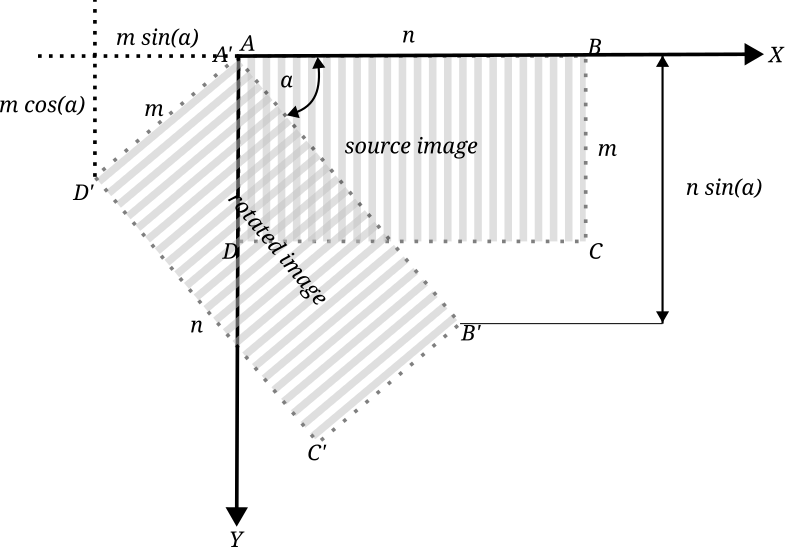
\includegraphics[width=0.4\textwidth]{rotation_example_1.png}
  \caption{Example demonstrating rotation of an image in the column major. Thus, every column vector of pixels are rotated at once (Represented by the strips in the image).}
  \label{fig:rotation_example_1}
\end{figure}

As seen in the example image in figure \ref{fig:rotation_example_1}, for the given angle of rotation, column vectors were rotated (represented by the stripes). Each such vector to be rotated begins from the line $\overrightarrow{A'B'}$. As such, the initial coordinates of each of these vectors can be determined by the equation of the same line, which is given by:
\begin{equation}
  \label{start_line_eq}
  f(i) = \left\lfloor \frac{i}{tan(\alpha)} \right\rfloor \forall \{i \in \mathbb{Z},\> i \in \left[ 0, n \cdot sin(\alpha) \right)\}
\end{equation}
Thus, the initial coordinates of the column vectors would be of the type $(f(i), i)$. Next, to determine the coordinates of the rest of the pixels in the column vector, as mentioned previously, we perform floating point addition or subtraction, depending on the extent to which each of the said vectors are spread across the coordinate axes.\\
In the example in figure \ref{fig:rotation_example_1}, we can see that each column vector is spread through a length of $m \cdot \sin(\alpha)$ in the $x$-axis and through a length of $m \cdot \cos(\alpha)$ in the $y$-axis. It may also be observed that these values are the projections of any line perpendicular to line defined by the function in equation \ref{start_line_eq} on the coordinate axes.\\
We now define:
$$\delta x = \left\lvert sin(\alpha)\right\rvert$$
$$\delta y = \left\lvert cos(\alpha)\right\rvert$$
The coordinates of the next pixel in the column vector is then given by:
$$(f(i) + \delta x, i + \delta y)$$
The coordinates of the pixel following that is determined by adding $\delta x$ and $\delta y$ to the previous coordinates accordingly, and so on, for each of the $m$ pixels in the given column vector. The end-result is that this operation covers all the $m \cdot \sin(\alpha)$ pixels in the $x$-axis and all the $m \cdot \cos(\alpha)$ pixels in the $y$-axis, therefore mapping all of the $m$ pixels in the specific column vector.\\
This process continues for all of the $n$ column vectors in the image, until the entire image is rotated. The signs for $\delta x$ and $\delta y$ depend on whether, while mapping the column vectors in the rotated image, the values of the $x$-coordinate $y$-coordinate are decreasing or increasing. In the given example in figure \ref{fig:rotation_example_1}, $\delta x$ is negative, but $\delta y$ is positive.\\
There is a third parameter, defined as:
$$\delta i = \frac{1}{\delta x}$$
$\delta i$ determines the rate at which the column vector is changed from one to the next, and its sign depends on the angle of rotation, $\alpha$.
The calculations for $\delta x$, $\delta y$, and $\delta i$ only happen once per column vector in the image, so the entire image transformation is quite fast, overall.

%%% TODO: DEFINE SUBSECTION FOR THE VERTICAL ROTATION THING
\subsection{Rotation Of An Image In The Row Major} \label{row_major_rotation}


% \begin{enumerate}[label=(\Alph*)]
% \end{enumerate}


% \begin{multicols}{2}
%   \begin{itemize}
%     \item \textbf{\textit{Zone 1}}, if $\alpha \in \left [ 0, \frac{\pi}{4} \right ]$
%     \item \textbf{\textit{Zone 2}}, if $\alpha \in \left ( \frac{\pi}{4}, \frac{\pi}{2} \right ]$
%     \item \textbf{\textit{Zone 3}}, if $\alpha \in \left ( \frac{\pi}{2}, \frac{3 \pi}{4} \right ]$
%     \item \textbf{\textit{Zone 4}}, if $\alpha \in \left ( \frac{3 \pi}{4}, \pi \right ]$
%   \end{itemize}
%   \vfill\null
%   \columnbreak
%   \begin{itemize}
%     \item \textbf{\textit{Zone 5}}, if $\alpha \in \left ( \pi, \frac{5 \pi}{4} \right ]$
%     \item \textbf{\textit{Zone 6}}, if $\alpha \in \left ( \frac{5 \pi}{4}, \frac{ 3 \pi}{2} \right ]$
%     \item \textbf{\textit{Zone 7}}, if $\alpha \in \left ( \frac{3 \pi}{2}, \frac{7 \pi}{4} \right ]$
%     \item \textbf{\textit{Zone 8}}, if $\alpha \in \left ( \frac{7 \pi}{4}, 2 \pi \right ]$
%   \end{itemize}
%   \vfill\null
%   \end{multicols}

% \subsection{Determining Start Line Equation}
% The start line equation varies from \textbf{\textit{zone}} to \textbf{\textit{zone}}.


\section{Conclusion}
The conclusion goes here.




% conference papers do not normally have an appendix


% use section* for acknowledgment
\section*{Acknowledgment}


The authors would like to thank...





% trigger a \newpage just before the given reference
% number - used to balance the columns on the last page
% adjust value as needed - may need to be readjusted if
% the document is modified later
%\IEEEtriggeratref{8}
% The "triggered" command can be changed if desired:
%\IEEEtriggercmd{\enlargethispage{-5in}}



  
%% references section
\bibliography{references} 
\bibliographystyle{ieeetr}

\end{document}
